%%
%% Automatically generated file from DocOnce source
%% (https://github.com/hplgit/doconce/)
%%

% #define PREAMBLE

% #ifdef PREAMBLE
%-------------------- begin preamble ----------------------

\documentclass[%
oneside,                 % oneside: electronic viewing, twoside: printing
final,                   % draft: marks overfull hboxes, figures with paths
10pt]{article}

\listfiles               %  print all files needed to compile this document

\usepackage{relsize,makeidx,color,setspace,amsmath,amsfonts,amssymb}
\usepackage[table]{xcolor}
\usepackage{bm,ltablex,microtype}

\usepackage[pdftex]{graphicx}

\usepackage[T1]{fontenc}
%\usepackage[latin1]{inputenc}
\usepackage{ucs}
\usepackage[utf8x]{inputenc}

\usepackage{lmodern}         % Latin Modern fonts derived from Computer Modern

% Hyperlinks in PDF:
\definecolor{linkcolor}{rgb}{0,0,0.4}
\usepackage{hyperref}
\hypersetup{
    breaklinks=true,
    colorlinks=true,
    linkcolor=linkcolor,
    urlcolor=linkcolor,
    citecolor=black,
    filecolor=black,
    %filecolor=blue,
    pdfmenubar=true,
    pdftoolbar=true,
    bookmarksdepth=3   % Uncomment (and tweak) for PDF bookmarks with more levels than the TOC
    }
%\hyperbaseurl{}   % hyperlinks are relative to this root

\setcounter{tocdepth}{2}  % levels in table of contents

% Tricks for having figures close to where they are defined:
% 1. define less restrictive rules for where to put figures
\setcounter{topnumber}{2}
\setcounter{bottomnumber}{2}
\setcounter{totalnumber}{4}
\renewcommand{\topfraction}{0.95}
\renewcommand{\bottomfraction}{0.95}
\renewcommand{\textfraction}{0}
\renewcommand{\floatpagefraction}{0.75}
% floatpagefraction must always be less than topfraction!
% 2. ensure all figures are flushed before next section
\usepackage[section]{placeins}
% 3. enable begin{figure}[H] (often leads to ugly pagebreaks)
%\usepackage{float}\restylefloat{figure}

% newcommands for typesetting inline (doconce) comments
\newcommand{\shortinlinecomment}[3]{{\color{red}{\bf #1}: #2}}
\newcommand{\longinlinecomment}[3]{{\color{red}{\bf #1}: #2}}

\usepackage[framemethod=TikZ]{mdframed}

% --- begin definitions of admonition environments ---

% Admonition style "mdfbox" is an oval colored box based on mdframed
% "notice" admon
\definecolor{mdfbox_notice_background}{rgb}{1,1,1}
\newmdenv[
  skipabove=15pt,
  skipbelow=15pt,
  outerlinewidth=0,
  backgroundcolor=mdfbox_notice_background,
  linecolor=black,
  linewidth=2pt,       % frame thickness
  frametitlebackgroundcolor=mdfbox_notice_background,
  frametitlerule=true,
  frametitlefont=\normalfont\bfseries,
  shadow=false,        % frame shadow?
  shadowsize=11pt,
  leftmargin=0,
  rightmargin=0,
  roundcorner=5,
  needspace=0pt,
]{notice_mdfboxmdframed}

\newenvironment{notice_mdfboxadmon}[1][]{
\begin{notice_mdfboxmdframed}[frametitle=#1]
}
{
\end{notice_mdfboxmdframed}
}

% Admonition style "mdfbox" is an oval colored box based on mdframed
% "summary" admon
\definecolor{mdfbox_summary_background}{rgb}{1,1,1}
\newmdenv[
  skipabove=15pt,
  skipbelow=15pt,
  outerlinewidth=0,
  backgroundcolor=mdfbox_summary_background,
  linecolor=black,
  linewidth=2pt,       % frame thickness
  frametitlebackgroundcolor=mdfbox_summary_background,
  frametitlerule=true,
  frametitlefont=\normalfont\bfseries,
  shadow=false,        % frame shadow?
  shadowsize=11pt,
  leftmargin=0,
  rightmargin=0,
  roundcorner=5,
  needspace=0pt,
]{summary_mdfboxmdframed}

\newenvironment{summary_mdfboxadmon}[1][]{
\begin{summary_mdfboxmdframed}[frametitle=#1]
}
{
\end{summary_mdfboxmdframed}
}

% Admonition style "mdfbox" is an oval colored box based on mdframed
% "warning" admon
\definecolor{mdfbox_warning_background}{rgb}{1,1,1}
\newmdenv[
  skipabove=15pt,
  skipbelow=15pt,
  outerlinewidth=0,
  backgroundcolor=mdfbox_warning_background,
  linecolor=black,
  linewidth=2pt,       % frame thickness
  frametitlebackgroundcolor=mdfbox_warning_background,
  frametitlerule=true,
  frametitlefont=\normalfont\bfseries,
  shadow=false,        % frame shadow?
  shadowsize=11pt,
  leftmargin=0,
  rightmargin=0,
  roundcorner=5,
  needspace=0pt,
]{warning_mdfboxmdframed}

\newenvironment{warning_mdfboxadmon}[1][]{
\begin{warning_mdfboxmdframed}[frametitle=#1]
}
{
\end{warning_mdfboxmdframed}
}

% Admonition style "mdfbox" is an oval colored box based on mdframed
% "question" admon
\definecolor{mdfbox_question_background}{rgb}{1,1,1}
\newmdenv[
  skipabove=15pt,
  skipbelow=15pt,
  outerlinewidth=0,
  backgroundcolor=mdfbox_question_background,
  linecolor=black,
  linewidth=2pt,       % frame thickness
  frametitlebackgroundcolor=mdfbox_question_background,
  frametitlerule=true,
  frametitlefont=\normalfont\bfseries,
  shadow=false,        % frame shadow?
  shadowsize=11pt,
  leftmargin=0,
  rightmargin=0,
  roundcorner=5,
  needspace=0pt,
]{question_mdfboxmdframed}

\newenvironment{question_mdfboxadmon}[1][]{
\begin{question_mdfboxmdframed}[frametitle=#1]
}
{
\end{question_mdfboxmdframed}
}

% Admonition style "mdfbox" is an oval colored box based on mdframed
% "block" admon
\definecolor{mdfbox_block_background}{rgb}{1,1,1}
\newmdenv[
  skipabove=15pt,
  skipbelow=15pt,
  outerlinewidth=0,
  backgroundcolor=mdfbox_block_background,
  linecolor=black,
  linewidth=2pt,       % frame thickness
  frametitlebackgroundcolor=mdfbox_block_background,
  frametitlerule=true,
  frametitlefont=\normalfont\bfseries,
  shadow=false,        % frame shadow?
  shadowsize=11pt,
  leftmargin=0,
  rightmargin=0,
  roundcorner=5,
  needspace=0pt,
]{block_mdfboxmdframed}

\newenvironment{block_mdfboxadmon}[1][]{
\begin{block_mdfboxmdframed}[frametitle=#1]
}
{
\end{block_mdfboxmdframed}
}

% --- end of definitions of admonition environments ---

% prevent orhpans and widows
\clubpenalty = 10000
\widowpenalty = 10000

% --- end of standard preamble for documents ---


\usepackage[swedish]{babel}

\raggedbottom
\makeindex
\usepackage[totoc]{idxlayout}   % for index in the toc
\usepackage[nottoc]{tocbibind}  % for references/bibliography in the toc

%-------------------- end preamble ----------------------

\begin{document}

% matching end for #ifdef PREAMBLE
% #endif

\newcommand{\exercisesection}[1]{\subsection*{#1}}

% This file is to be run by preprocess to produce newcommands.tex
% to be included in .tex files.
% There are format-specific tests here for the newcommands (i.e.,
% different definitions of the commands depending on latex or mathjax).

% Newcommands for LaTeX math.
\newcommand{\tp}{\thinspace .}
\renewcommand{\Re}{\bbbr}
\newcommand{\Oof}[1]{\mathcal{O}(#1)}
\newcommand{\Prob}[1]{\hbox{P}(#1)}
\newcommand{\Var}[1]{\hbox{Var}(#1)}
\newcommand{\Cov}[2]{\hbox{Cov}(#1,#2)}
\newcommand{\StDev}[1]{\hbox{StDev}(#1)}

\newcommand{\punkt}{\thinspace .}
\newcommand{\komma}{\thinspace ,}

\newcommand{\vr}{\vec{r}}
\newcommand{\vrp}{\vec{r}\,'}
\newcommand{\erf}{\mathrm{erf}}
\newcommand{\vrho}{\vec{\varrho}}
\newcommand{\vrhop}{\vec{\varrho}\, '}
\newcommand{\sign}{\mathrm{sign}}

\newcommand{\Tr}[1]{\mathrm{Tr}[#1]}
\newcommand{\e}{\varepsilon}
\newcommand{\g}{\gamma}

\newcommand{\half}{\frac{1}{2}}
\newcommand{\vnabla}{\vec{\nabla}}


% Use footnotesize in subscripts
\newcommand{\subsc}[2]{#1_{\mbox{\footnotesize #2}}}




% ------------------- main content ----------------------



% ----------------- title -------------------------

\thispagestyle{empty}

\begin{center}
{\LARGE\bf
\begin{spacing}{1.25}
FFM234, Klassisk fysik och vektorfält - Föreläsningsanteckningar
\end{spacing}
}
\end{center}

% ----------------- author(s) -------------------------

\begin{center}
{\bf \href{{http://fy.chalmers.se/subatom/tsp/}}{Christian Forssén}, Institutionen för fysik, Chalmers, Göteborg, Sverige${}^{}$} \\ [0mm]
\end{center}

\begin{center}
% List of all institutions:
\end{center}
    
% ----------------- end author(s) -------------------------

% --- begin date ---
\begin{center}
Oct 4, 2019
\end{center}
% --- end date ---

\vspace{1cm}


\section*{8. Potentialteori}

\subsection*{Konservativa fält och potentialer}

Vi har definierat ett konservativt fält som ett fält $\vec{F}$ sådant att
\begin{equation}
  \oint_C \vec{F}\cdot \mbox{d}\vec{r} = 0
\end{equation}
för varje sluten kurva $C$.  Enligt Stokes sats följer det nu att ett fält som har $\vnabla \times \vec{F} = 0$ överallt i ett enkelt sammanhängande område är konservativt. Vi har sedan antagit att vi kan skriva
\begin{equation}
\vec{F} = - \vnabla \phi,
\end{equation}
där $\phi$ kallas för det konservativa fältets potential. Gäller då 
$$
\vnabla \times \vec{F} = 0 \, \Longleftrightarrow \, \vec{F} = - \vnabla \phi \, ??
$$
Nej, det har vi ännu inte visat! Vi har att $\vec{F} = - \vnabla \phi \, \Rightarrow \, \vnabla \times \vec{F} = 0 \, \Rightarrow \, \oint_C \vec{F}\cdot \mbox{d}\vec{r} = 0$ eftersom $\vnabla \times ( \vnabla \phi) = 0$ (se nedan), men det omvända gäller inte per automatik. Vi har ännu inte visat att konservativa fält alltid kan skrivas som $-\vnabla \phi$.


\begin{notice_mdfboxadmon}[Bevis av $\vnabla \times ( \vnabla \phi) = 0$ mha indexnotation]
Vi kan visa att $\vnabla \times ( \vnabla \phi) = 0$ mha indexnotation: Vektorn $\left[ \vnabla \times ( \vnabla \phi) \right]_i = \epsilon_{ijk} \partial_j \partial_k \phi = 0$ eftersom den resulterande summan med nio termer $\sum_{j,k=1}^3$ har två nollskilda som tar ut varandra. T.ex. för $i=1$ fås $\partial_2\partial_3 \phi - \partial_3\partial_2 \phi = 0$.
\end{notice_mdfboxadmon} % title: Bevis av $\vnabla \times ( \vnabla \phi) = 0$ mha indexnotation



Definitionen av ett konservativt fält gör dock att vi kan hitta en potential från
\begin{equation}
  \int_{\vec{r}_1}^{\vec{r}_2} \vec{F} \cdot \mbox{d} \vec{r} = \phi\left( \vec{r}_1 \right) - \phi\left( \vec{r}_2 \right) = - \int_{\vec{r}_1}^{\vec{r}_2} \mbox{d} \phi.
\end{equation}
Notera tecknet på potentialskillnaden i HL. Det hade gått lika bra med det omvända, men just denna konvention stämmer överens med energitolkningen i klassisk mekanik.

Vi ser nu att förändringen av potentialen mellan punkterna $\vec{r}$ och $\vec{r} + \mbox{d}\vec{r}$ är
\begin{equation}
  \mbox{d}\phi = -\vec{F}\cdot \mbox{d}\vec{r},
\end{equation}
men denna förändring kan också skrivas som
\begin{equation}
  \mbox{d}\phi = \vnabla \phi \cdot \mbox{d}\vec{r}.
\end{equation}
Det följer därmed att det finns en potential $\phi$ så att det konservativa fältet $\vec{F}$ kan skrivas
\begin{equation}
  \vec{F} = -\vnabla \phi.
\end{equation}
Faktum är att $\phi$ inte är entydigt bestämd.  Man kan skapa en ny potential genom att addera en konstant till en potential: $\phi \mapsto \phi + \phi_0$.


\begin{notice_mdfboxadmon}[Exempel: Arbete i klassisk mekanik]

För ett konservativt kraftfält $\vec{F}$ gäller att det uträttade arbetet längs en rörelsebana motsvarar en \emph{ökning} av den kinetiska energin åtföljt av en motsvarade \emph{minskning} av en potentiell energi så att den totala mekaniska energin $E = T + V$ är \emph{konserverad}.

\longinlinecomment{Kommentar 1}{ Notera att uträttat arbete kan vara negativt vilket isf innebär en minskning av den kinetiska energin och en ökning av den potentiella. }{ Notera att uträttat arbete }

Arbetet som uträttas längs en kurva $C$ motsvaras av kurvintegralen
\begin{align}
\int_C \vec{F} \cdot \mbox{d}\vec{r} &= \left\{ \begin{array}{l}
\vec{F} = m \vec{a} = m \frac{\mbox{d}\vec{v}}{\mbox{d}t} \\
\mbox{d}\vec{r} = \vec{v} \mbox{d}t
\end{array} 
, \quad \frac{\mbox{d}\vec{v}}{\mbox{d}t} \cdot \vec{v} = \frac{1}{2}\frac{\mbox{d}}{\mbox{d}t} (\vec{v} \cdot \vec{v})
\right\} \\
&= \frac{m}{2} \int_{t_A}^{t_B} \frac{\mbox{d}}{\mbox{d}t} (\vec{v} \cdot \vec{v}) \mbox{d}t = \frac{m v_2^2}{2} - \frac{m v_1^2}{2} = \delta T.
\end{align}
Här har vi använt NII. Tidpunkterna $t_A$ och $t_B$ motsvarar start- respektive sluttiden för rörelsen.

Ett exempel på ett sådant konservativt kraftfält är gravitationskraften nära jordytan: $\vec{F} = - m g \hat{z}$.
Med vår nuvarande kunskap skulle vi uttrycka detta som $\vec{F} = -\vnabla \phi$, där vi alltså använder beteckningen $\phi$ istället för $V$. För vårt exempel finner vi att potentialen $\phi(\vec{r}) = m g z$ uppfyller denna likhet.

Vidare uppfyller kraftfältet $\vnabla \times \vec{F} = 0$. Vi kontrollerar detta för vårt exempel: 
$$
\begin{vmatrix}
\hat{x} & \hat{y} & \hat{z} \\
\frac{\partial}{\partial x} & \frac{\partial}{\partial y} & \frac{\partial}{\partial z} \\
\mbox{0}  &  \mbox{0}  & -mg \\
\end{vmatrix}
= 0
$$

Kurvintegralen
$$
\int_C \vec{F} \cdot \mbox{d}\vec{r} = \phi\left( \vec{r}_A \right) - \phi\left( \vec{r}_B \right),
$$
där $A$ och $B$ är kurvans start- respektive slutpunkt. Här finner vi att potentialskillnaden $-\delta \phi = \phi(z_A) - \phi(z_B) = mg (z_A-z_B)$. Detta är alltså den negativa skillnaden i potentiell energi och vi får
$$
\delta T = - \delta \phi \quad \Rightarrow \quad \delta(T+V) = 0.
$$
\end{notice_mdfboxadmon} % title: Exempel: Arbete i klassisk mekanik



\subsection*{Poissons och Laplaces ekvationer}

Konservativa vektorfält är alltså rotationsfria, men de kan fortfarande ha nollskild divergens. Denna kallas ofta för \emph{källtäthet}
\begin{equation}
\rho(\vec{r}) = \vnabla \cdot \vec{F}.
\end{equation}


\begin{warning_mdfboxadmon}[Kommentar]
Låt oss använda superposition och deltafunktioner för att visa att $\vnabla \cdot \vec{F} = \rho(\vec{r})$. Superposition ger oss potentialen från en laddningsfördelning på integralform
$$
\phi(\vec{r}) = \frac{1}{4\pi} \int \frac{1}{\left| \vec{r} - \vec{r}\,' \right|} \rho(\vec{r}\,') dV'.
$$
eller det motsvarande fältet (notera att $\vnabla$ opererar på $\vec{r}$)
$$
\vec{F}(\vec{r}) = -\vnabla \phi(\vec{r}) = \frac{1}{4\pi} \int \frac{\vec{r} - \vec{r}\,'}{\left| \vec{r} - \vec{r}\,' \right|^3} \rho(\vec{r}\,') dV'.
$$
Beräkna nu divergensen av ovanstående (notera att den opererar på $\vec{r}$), och identifiera deltafunktionen
$$
\vnabla \cdot \vec{F} = \frac{1}{4\pi} \int \vnabla \cdot \left( \frac{\vec{r} - \vec{r}\,'}{\left| \vec{r} - \vec{r}\,' \right|^3}\right) \rho(\vec{r}\,') dV'
= \frac{1}{4\pi} \int 4\pi \delta( \vec{r} - \vec{r}\,' ) \rho(\vec{r}\,') dV' = \rho(\vec{r}).
$$
\end{warning_mdfboxadmon} % title: Kommentar




Med $\vec{F} = -\vnabla \phi$ får vi \emph{Poissons ekvation}
\begin{equation}
\vnabla \cdot \vnabla \phi(\vec{r}) = \Delta \phi(\vec{r}) = -\rho(\vec{r}),
\end{equation}
vilket alltså ger potentialen på differentialform.

Specialfallet av denna ekvation utan källa, dvs divergensfritt, ger \emph{Laplaces ekvation}
\begin{equation}
\Delta \phi(\vec{r}) = 0.
\end{equation}
Kom ihåg att $\Delta$ är Laplacianen vilken kan skrivas
\begin{equation}
\Delta \phi = \left( \frac{\partial^2}{\partial x^2} + \frac{\partial^2}{\partial y^2} + \frac{\partial^2}{\partial z^2} \right) \phi,
\end{equation}
i Cartesiska koordinater. Den ser annorlunda ut i kroklinjiga koordinatsystem.


\begin{warning_mdfboxadmon}[Kommentar]
Notera att $\vec{F} = -m g \hat{z}$ är divergensfritt och att potentialen $\phi = m g z$ uppfyller Laplaces ekvation $\Delta \phi = 0$.
\end{warning_mdfboxadmon} % title: Kommentar



Notera att Poissons och Laplaces ekvationer är exempel på \emph{differentialekvationer}. För att lösa dessa i ett område behöver man också veta randvillkor för fältet $\phi$. 

Vi kommer t.ex. se att (ett stationärt) temperaturfält uppfyller någon av dessa ekvationer (Laplaces ekvation om det inte finns en värmekälla). För att t.ex. räkna ut temperaturfältet inuti ett värmeisolerande fönster behöver vi veta randvillkor för fältet på glasets in- och utsida.

Olika tekniker för lösning av dessa ekvationer presenteras i kapitel 9.


\begin{warning_mdfboxadmon}[Integral- och differentialform för potentialen]
Sammanfattningsvis kan vi uttrycka potentialen $\phi(\vec{r})$ för ett konservativt fält på två olika sätt utgående från dess källtäthet $\rho(\vec{r})$. 
\begin{itemize}
\item Dels på integralform enligt superpositionsprincipen
\end{itemize}

\noindent
\[
\phi(\vec{r}) = \frac{1}{4\pi} \int \frac{1}{\left| \vec{r} - \vec{r}\,' \right|} \rho(\vec{r}\,') dV'.
\] 
\begin{itemize}
\item Dels på differentialform enligt Poissons ekvation
\end{itemize}

\noindent
\[
\Delta \phi(\vec{r}) = -\rho(\vec{r}).
\]
Vi kommer dock att behöva prata mer om \emph{randvillkor}.
\end{warning_mdfboxadmon} % title: Integral- och differentialform för potentialen




\subsection*{Divergensfria fält}

Kan man erhålla \emph{divergensfria} fält från någon potential på liknande sätt som vi just gjorde för rotationsfria fält?

Vi betraktar ett divergensfritt fält $\vec{G}$
$$
\vnabla \cdot \vec{G} = 0,
$$
och nöjer oss med att konstatera att divergensfriheten uppenbarligen uppfylls om fältet kan skrivas
\begin{equation}
\vec{G} = \vnabla \times \vec{A}.
\end{equation}

\longinlinecomment{Kommentar 2}{ Visa detta om ni är osäkra.   Gärna med indexnotation. $$ \vnabla \cdot (\vnabla \times \vec{A}) = \partial_i \epsilon_{ijk} \partial_j A_k, $$ Vilket är en summa med 27 termer, vara sex är nollskilda och dessa tar ut varandra parvis.  Alternativt med Stokes och Gauss satser: Betrakta volymsintegralen av $\vnabla \cdot \vec{G}$, och beräkna normalytintegralen av $\vec{G} = \vnabla \times \vec{A}$ över randytan genom att dela upp den i två delar och applicera Stokes sats på varje del. Notera att dessa två ytor kommer att ha samma rand, men motsatt riktning. Slutsatsen blir att $\vnabla \cdot \vec{G} = 0$. }{ Visa detta om ni }

Vektorfältet $\vec{A}$ kallas då för en \emph{vektorpotential}.


\begin{notice_mdfboxadmon}[Standardexempel: Statiskt magnetfält]

Ett statiskt magnetfält $\vec{B}(\vec{r})$ är divergensfritt och uppfyller $\vec{B}(\vec{r}) = \vnabla \times \vec{A}(\vec{r})$ där $\vec{A}$ kallas för den elektromagnetiska vektorpotentialen.
\end{notice_mdfboxadmon} % title: Standardexempel: Statiskt magnetfält



Vi fann tidigare att skalära potentialer hade en invarians genom att vi kunde addera en konstant term $\phi \mapsto \phi + \phi_0$ utan att ändra fältstyrkan.

På samma sätt har vektorpotentialen en invarians
\begin{equation}
\vec{A}(\vec{r}) \mapsto \vec{A}(\vec{r}) + \vnabla \Lambda(\vec{r}),
\end{equation}
där $\Lambda$ kallas för en Gaugeparameter och invariansen kallas för \emph{Gaugeinvarians}. 


\begin{warning_mdfboxadmon}[Kommentar]
Detta må verka som en kuriositet, men just Gaugeinvarians är av fundamental betydelse för vår teoretiska förståelse av elektromagnetiska, svaga och starka krafter.
\end{warning_mdfboxadmon} % title: Kommentar




\begin{warning_mdfboxadmon}[Kommentar]
Ofta använder man Gaugeinvariansen till att skapa en vektorpotential som är divergensfri. Dvs man väljer $\Lambda$ så att $\Delta \Lambda = -\vnabla \cdot \vec{A}$.
\end{warning_mdfboxadmon} % title: Kommentar



Rotationen kallas ofta för virveltäthet
$$
\vnabla \times \vec{G} = \vec{j} \quad \Rightarrow \vnabla \times (\vnabla \times \vec{A}) = \vec{j}.
$$
Vi använder sambandet $\vnabla \times \left( \vnabla \times \vec{A} \right) = \vnabla \left( \vnabla \cdot \vec{A} \right) - \Delta \vec{A}$ vilket alltså ger
$$
\Delta \vec{A} - \vnabla \left( \vnabla \cdot \vec{A} \right) = -\vec{j}.
$$
Genom att välja Gaugeparametern så att $\vnabla \cdot \vec{A} = 0$ får vi Poissons ekvation för vektorpotentialen
\begin{equation}
\Delta \vec{A} = -\vec{j}.
\end{equation}

\subsection*{Potentialer för godtyckliga vektorfält}

\begin{itemize}
\item Betrakta ett fält med både källor och virvlar, dvs $\vnabla \cdot \vec{H} = \rho \neq 0$ och $\vnabla \times \vec{H} = \vec{j} \neq 0$.

\item Detta allmänna vektorfält kan vi dela upp i två delar $\vec{H} = \vec{F} + \vec{G}$ där
\end{itemize}

\noindent
\begin{align}
\vnabla \cdot \vec{F} &= \rho \quad  &\vnabla \cdot \vec{G} &= 0 \\
\vnabla \times \vec{F} &= 0 \quad  &\vnabla \times \vec{G} &= \vec{j}
\end{align}

\begin{itemize}
\item Dvs, fältet $\vec{H}$ kan skrivas som summan av ett rotationsfritt fält $\vec{F}$ och ett divergensfritt fält $\vec{G}$ som representeras av potentialerna $\phi$ och $\vec{A}$.
\end{itemize}

\noindent
$$
\vec{H} = \vec{F} + \vec{G} = -\vnabla \phi + \vnabla \times \vec{A}.
$$


\begin{notice_mdfboxadmon}[Exempel: Stagnationsström konservativt hastighetsfält]

Betrakta (det rotationsfria) hastighetsfältet som ges av potentialen
$$
\phi(x,y) = \frac{A}{2}(x^2 - y^2),
$$
där $A$ är en positiv konstant. Hastighetsfältet blir
$$
\vec{v} = -\vnabla \phi \quad \Rightarrow 
\left\{
\begin{array}{l}
v_x = -A x \\
v_y = A y
\end{array}
\right.
$$
Vi noterar att detta fält också är divergensfritt. 

En fältbild (potential och fältlinjer) visas nedan. Notera att det finns områden där hastigheten är noll. Dessa kallas stagnationspunkter. Vi noterar också att fältlinjerna blir parallella med $x$- och $y$-axlarna när vi kommer tillräckligt nära. Vi kan därför tänka oss dessa som fasta väggar och att vårt hastighetsfält beskriver strömmen vid ett hörn.



\vspace{6mm}

% inline figure
\centerline{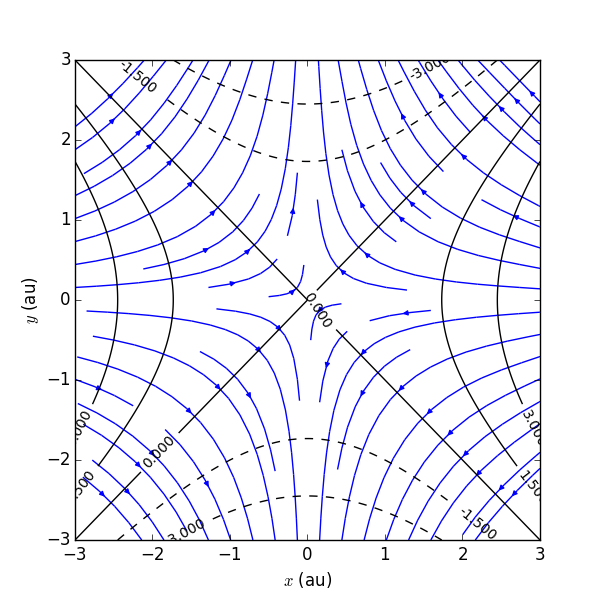
\includegraphics[width=0.8\linewidth]{fig/stagnation_fieldplot.png}}

\vspace{6mm}



I verkligheten kommer dock friktionen nära väggen att skapa virvlar, och vår rotationsfria approximation ger en sämre beskrivning.
\end{notice_mdfboxadmon} % title: Exempel: Stagnationsström konservativt hastighetsfält



\subsection*{Standardexempel på käll- och virvelfördelningar}

\paragraph{Punktkälla med styrkan $q$ i origo.}
\begin{itemize}
\item vektorfält 
\end{itemize}

\noindent
$$
\vec F=\frac{q}{4\pi r^2}\hat r.
$$
\begin{itemize}
\item rotationsfritt, men med en källa $\rho=q\delta^3(\vec{r})$. Fältet har en potential
\end{itemize}

\noindent
$$
\phi=\frac{q}{4\pi r},
$$
som uppfyller Poissons ekvation med källan $\rho=q\delta^3(\vec{r})$, 
$$
\Delta\phi=-q\delta^3(\vec{r}).
$$

\paragraph{Linjekälla på $z$-axeln med konstant styrka $k$.}
\begin{itemize}
\item vektorfält
\end{itemize}

\noindent
$$
\vec F=\frac{k}{2\pi\varrho}\hat\varrho
$$
\begin{itemize}
\item Motsvarande potential är 
\end{itemize}

\noindent
$$
\phi=-\frac{k}{2\pi}\log\frac{\varrho}{\varrho_0},
$$
\begin{itemize}
\item Potentialen uppfyller Poissons ekvation:
\end{itemize}

\noindent
$$
\Delta\phi=-k\delta^2(\vec{\varrho}).
$$

\paragraph{Virveltråd på $z$-axeln med styrka $J$.}
\begin{itemize}
\item fältet 
\end{itemize}

\noindent
$$
\vec G=\frac{J}{2\pi\varrho}\hat\varphi.
$$
\begin{itemize}
\item Vektorpotentialen är (t.ex., med tanke på gaugeinvarians)
\end{itemize}

\noindent
$$
\vec A=-\frac{J\hat z}{2\pi}\log\frac{\varrho}{\varrho_0},
$$
(kontrollera; $\vnabla\times\vec A$ i cylindriska koordinater)
$$
\vnabla\times\vec A=\frac{1}{\varrho}
	\begin{vmatrix}
        \hat\varrho & \varrho\hat\varphi & \hat z \\ \frac{\partial}{\partial \varrho} & 
\frac{\partial}{\partial \varphi} &
        \frac{\partial}{\partial z} \\ 0\mbox{} & 0\mbox{} & -\frac{J}{2\pi}\log\varrho \\
        \end{vmatrix}
           =\frac{J}{2\pi\varrho}\hat\varphi.
$$
\begin{itemize}
\item Notera att denna vektorpotential uppfyller $\vnabla\cdot\vec A=0$, och därför ges virvelfördelningen av 
\end{itemize}

\noindent
$$
\vnabla \times \vec{G} = \vec{\jmath} = -\Delta\vec A.
$$ 
\begin{itemize}
\item Poissons ekvation, 
\end{itemize}

\noindent
$$
\Delta\vec A=-J\hat z\delta^2(\vec{\varrho}).
$$


\subsection*{Randvärdesproblem}

En lösning av t.ex. Laplaces ekvation $\Delta \phi = 0$ ger upphov till integrationskonstanter. För att entydigt bestämma lösningen behövs därför \emph{randvillkor} för fältet.


\begin{warning_mdfboxadmon}[Rita]
Skissa gärna hur ett fält som uppfyller Laplaces ekvation beter sig. 

Lösningarna är så kallade harmoniska funktioner. Villkoret $\Delta \phi = 0$ ger att det inte finns några extrempunkter inuti området, dvs maximum och minimum måste ligga på randen.

Titta på ett fält $\phi(x,y)$ och använd Taylorexpansion för att teckna beteendet \emph{nära} en punkt $\vec{r}_0$
\begin{align*}
\phi(\vec{r}) =  &c_0 + c_x (x-x_0) + c_y (y-y_0) \\
&+ c_{xy} (x-x_0)(y-y_0)+ \frac{c_{xx}}{2}(x-x_0)^2 + \frac{c_{yy}}{2}(y-y_0)^2 +\ldots,
\end{align*}
där t.ex. $c_0 = \phi(\vec{r}_0)$, $c_x = \left. \frac{d\phi}{dx} \right|_{\vec{r} = \vec{r}_0}$, etc. 

Villkoret $\frac{\partial^2\phi}{\partial x^2} + \frac{\partial^2\phi}{\partial y^2} = 0$ (överallt) betyder att $c_{xx} = -c_{yy}\equiv c_{ii}$ samt att alla högre ordningens termer måste vara noll. 

Det viktiga är alltså att expansionen slutar med den kvadratiska termen och att dessa är lika, men motriktade, i $x$- och $y$-led. De specifika värdena på konstanterna $(c_0, c_x, c_y,c_{xy},c_{ii})$ kommer förstås att bero på vilken punkt $\vec{r}_0$ som vi använder för Taylorexpansionen.
\end{warning_mdfboxadmon} % title: Rita



\paragraph{Exempel: Lösningar till Laplaces ekvation.}
\begin{figure}[!ht]  % fig:xy
  \centerline{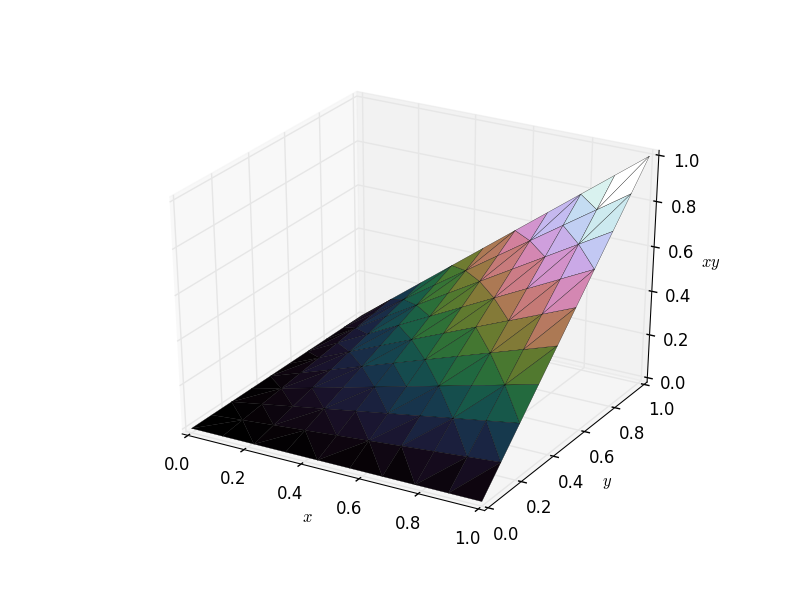
\includegraphics[width=0.8\linewidth]{fig/xy.png}}
  \caption{
  Lösningen ($\phi = xy$) till Laplaces ekvation i två dimensioner på ett kvadratiskt område med randvillkor enligt figuren. \label{fig:xy}
  }
\end{figure}
%\clearpage % flush figures fig:xy



\begin{figure}[!ht]  % fig:x2y2
  \centerline{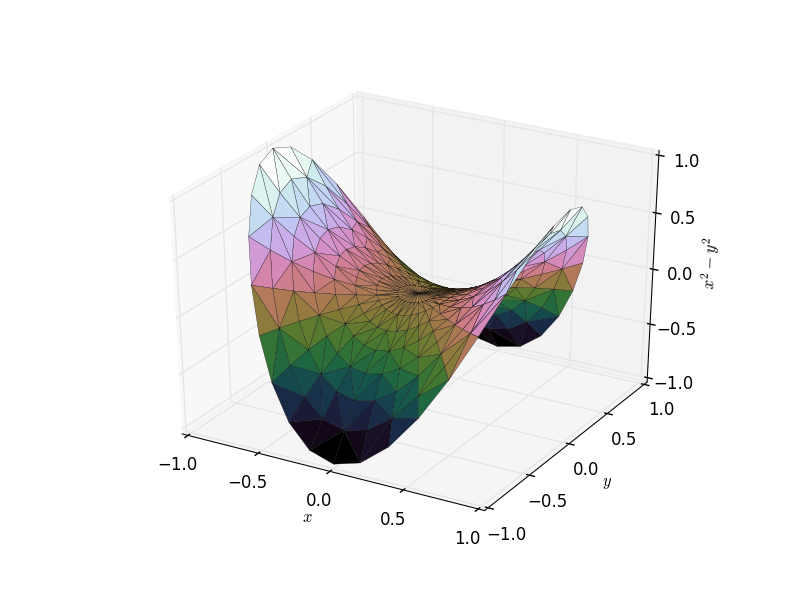
\includegraphics[width=0.8\linewidth]{fig/x2y2.png}}
  \caption{
  Lösningen ($\phi = x^2 - y^2$) till Laplaces ekvation i två dimensioner på ett cirkulärt område med vinkelberoende randvillkor enligt figuren. \label{fig:x2y2}
  }
\end{figure}
%\clearpage % flush figures fig:x2y2


Två exempel på lösningar till Laplaces ekvation i ett område med givna randvillkor visas i figurerna~\ref{fig:xy} och~\ref{fig:x2y2}.



\begin{warning_mdfboxadmon}[Kommentar]
Att ta reda på precis ``hur mycket'' villkor, och av vilket slag, man bör lägga på fältet på randen $\partial V$ är ju ett matematiskt problem, men det matematiska svaret på frågan bör också vara ett svar inom fysik, så att en given fysikalisk förutsättning ger en unik lösning (fältkonfiguration).
\end{warning_mdfboxadmon} % title: Kommentar



\begin{itemize}
\item Vårt randvärdesproblem består av den partiella differentialekvationen $\Delta\phi=-\rho$ samt några randvillkor. 

\item Vilka randvillkor ger en \emph{unik} lösning? Eller hur skall ``bra'' randvillkor formuleras? 

\item Antag att $\phi_1$ och $\phi_2$ båda är lösningar. 

\item $\psi=\phi_1-\phi_2$, uppfyller Laplaces ekvation, $\Delta\psi=0$. 

\item En trivial lösning, $\psi=\mathrm{konstant}$, innebär att lösningen till Poissons ekvation är unik.
\end{itemize}

\noindent
\shortinlinecomment{Kommentar 3}{ Eftersom $\phi_1$ och $\phi_2$ ger samma vektorfält om de enbart skiljer på en konstant. }{ Eftersom $\phi_1$ och $\phi_2$ }

Betrakta nu identiteten
$$
\vnabla\cdot(\psi\vnabla\psi)=\vnabla\psi\cdot\vnabla\psi+\psi\Delta\psi
=\vnabla\psi\cdot\vnabla\psi=|\vnabla\psi|^2,
$$
som gäller när $\Delta\psi=0$. Tillämpa nu Gauss sats på vektorfältet $\psi\vnabla\psi$. 
$$
\int_{\partial V}\psi\vnabla\psi\cdot d\vec S = \int_V \vnabla\cdot(\psi\vnabla\psi) dV = \int_V|\vnabla\psi|^2dV.
$$
\begin{itemize}
\item HL är positivt semidefinit, och noll endast om $\psi = \mathrm{konstant}$. 

\item Randvillkor som gör VL till noll innebär därför det vi vill.
\end{itemize}

\noindent
Ytintegralen i VL är 
$$
\int_{\partial V}\psi(\vnabla\psi\cdot\hat n)dS.
$$ 
Två faktorer i integranden: $\psi$ och $\vnabla\psi\cdot\hat n$. 

\shortinlinecomment{Kommentar 4}{ Den andra faktorn är ``normalderivatan'' vid randen, alltså riktningsderivatan i normalens riktning. }{ Den andra faktorn är }

\shortinlinecomment{Kommentar 5}{ Lösningen till Laplaces ekvation är trivial (konstant) om den ena eller den andra är noll på randen. }{ Lösningen till Laplaces ekvation }

\paragraph{Dirichlets randvillkor:}
$$
\psi = 0 \mathrm{~på~} \partial V \quad \Rightarrow \quad \psi = 0 \mathrm{~i~} V
$$
Detta ger att lösningen $\phi_1 = \phi_2$ på randen, dvs
$$
\phi|_{\partial V}=f,
$$
där $f$ är en funktion på randen

\paragraph{Neumanns randvillkor:}
$$
(\vnabla\psi) \cdot \hat n=0 \mathrm{~på~} \partial V \quad \Rightarrow \quad \psi = \mathrm{konstant} \mathrm{~i~} V
$$
Detta ger att $(\vnabla\phi_1) \cdot \hat n=(\vnabla\phi_2) \cdot \hat n$ på randen, dvs
$$
(\vnabla\phi)|_{\partial V}\cdot\hat n=g,
$$
där $g$ är en funktion på randen. 

\paragraph{Sammanfattning:}
Poissons ekvation i volymen $V$ med någon källfördelning $\rho$ har en unik lösning (sånär
som på en ointressant konstant) för dessa två typer av randvillkor.

% ------------------- end of main content ---------------

% #ifdef PREAMBLE
\end{document}
% #endif

